\documentclass[11pt]{report}
% this template is originally from Roy Dong's ECE 515.
% Edited by Dawei Sun
%%%%%%%%%%%%%%%%%%%%%%%%%%%%%%%%%%%%%%%%%%%%%%%%%%%%%%%%%%%%%%%%%%
% Set the margins of our document.
\usepackage[margin = 1 in]{geometry}

%%%%%%%%%%%%%%%%%%%%%%%%%%%%%%%%%%%%%%%%%%%%%%%%%%%%%%%%%%%%%%%%%%
% Import commands for custom header.
\usepackage{fancyhdr}
\pagestyle{fancy}

%%%%%%%%%%%%%%%%%%%%%%%%%%%%%%%%%%%%%%%%%%%%%%%%%%%%%%%%%%%%%%%%%%
% Allow ourselves to do equations!
\usepackage{amsmath,amssymb,amsthm,amsfonts}
\usepackage{upgreek}
\usepackage{mathtools}
\usepackage{bbm}
\usepackage{hyperref}

%%%%%%%%%%%%%%%%%%%%%%%%%%%%%%%%%%%%%%%%%%%%%%%%%%%%%%%%%%%%%%%%%%
% Nicer formatting for enumerate commands.
\usepackage[shortlabels]{enumitem}

\usepackage{algorithm2e}
\usepackage[noend]{algpseudocode}

%%%%%%%%%%%%%%%%%%%%%%%%%%%%%%%%%%%%%%%%%%%%%%%%%%%%%%%%%%%%%%%%%%
% Colored text and include images.
\usepackage{color}
\usepackage[dvipsnames]{xcolor}
\usepackage{graphicx}

\usepackage{listings}
\usepackage{multicol}
%%%%%%%%%%%%%%%%%%%%%%%%%%%%%%%%%%%%%%%%%%%%%%%%%%%%%%%%%%%%%%%%%%
% Some custom macros to make life easier.
\newcommand{\mc}{\mathcal}
\newcommand{\mb}{\mathbb}
\newcommand{\reals}{\mathbb{R}}

\newcommand{\T}{\intercal}
\newcommand{\E}[1]{\mathbb{E}\left[#1\right]}

%%%%%%%%%%%%%%%%%%%%%%%%%%%%%%%%%%%%%%%%%%%%%%%%%%%%%%%%%%%%%%%%%%
%%%%%%%%%%%%%%%%%%%%%%%%%%%%%%%%%%%%%%%%%%%%%%%%%%%%%%%%%%%%%%%%%%
%%%%%%%%%%%%%%%%%%%%%%%%%%%%%%%%%%%%%%%%%%%%%%%%%%%%%%%%%%%%%%%%%%

\lhead{ECE 553 - Fall 2020 at University of Illinois at Urbana-Champaign}
\rhead{\textcolor{red}{Dawei Sun (daweis2)}}

%%%%%%%%%%%%%%%%%%%%%%%%%%%%%%%%%%%%%%%%%%%%%%%%%%%%%%%%%%%%%%%%%%
%%%%%%%%%%%%%%%%%%%%%%%%%%%%%%%%%%%%%%%%%%%%%%%%%%%%%%%%%%%%%%%%%%
%%%%%%%%%%%%%%%%%%%%%%%%%%%%%%%%%%%%%%%%%%%%%%%%%%%%%%%%%%%%%%%%%%

\begin{document}

%%%%%%%%%%%%%%%%%%%%%%%%%%%%%%%%%%%%%%%%%%%%%%%%%%%%%%%%%%%%%%%%%%
%%%%%%%%%%%%%%%%%%%%%%%%%%%%%%%%%%%%%%%%%%%%%%%%%%%%%%%%%%%%%%%%%%
%%%%%%%%%%%%%%%%%%%%%%%%%%%%%%%%%%%%%%%%%%%%%%%%%%%%%%%%%%%%%%%%%%

\section*{Exercise 4.2}
\paragraph{From Lagrange to Mayer form.} The augmented system is as follows.
\begin{align*}
&y = \begin{bmatrix}x^0\\x_1\\x_2\end{bmatrix},~y_0 = \begin{bmatrix}0\\0\\0\end{bmatrix},~\dot{y} = \begin{bmatrix}1\\x_2\\u\end{bmatrix},\\
&H(x,u,p,p_0) = p_1 x_2 + p_2 u + p_0.
\end{align*}
Moreover, we know that $u^* \equiv 1$, $t^* = 2$, and $y^*(t^*) = \begin{bmatrix}2\\2\\2\end{bmatrix}$.
\paragraph{Temporal control perturbation.} Perturbed control is shown in Fig.~\ref{fig:temporal_control_perturbation}. Numerical evaluation gives that $\delta(\tau) = g(y^*(t^*), u^*(t^*))\tau = \begin{bmatrix}1\\2\\1\end{bmatrix}\tau$.
\begin{figure}[H]
    \centering
    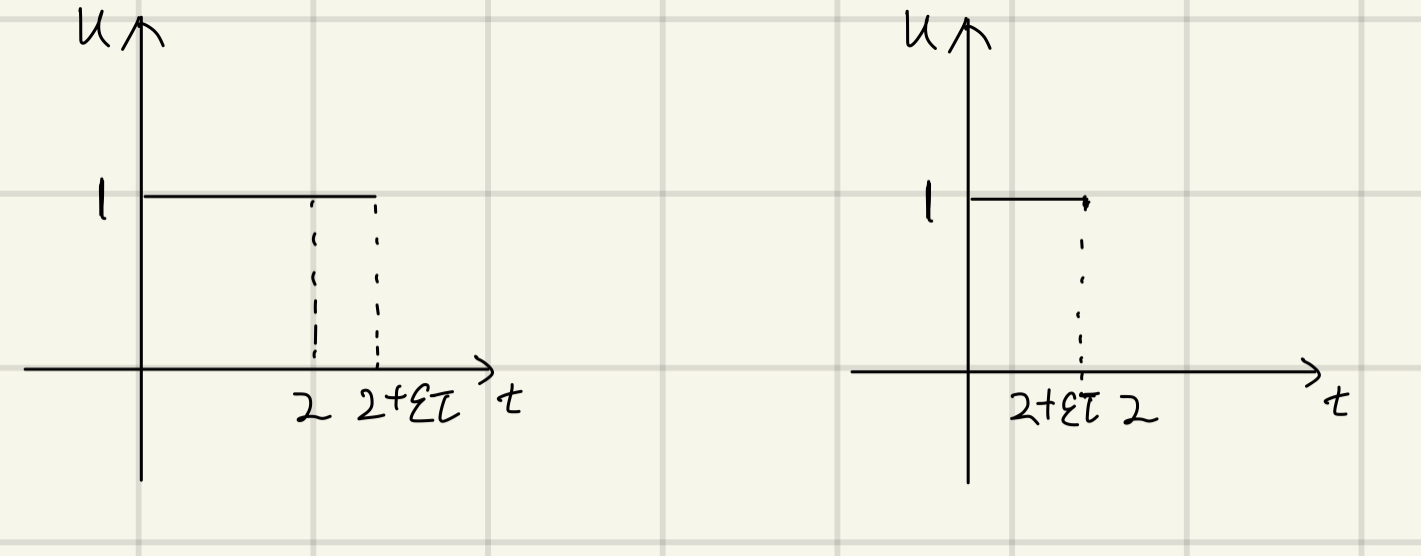
\includegraphics[width=\textwidth]{ECE553/hw6/IMG_0040.PNG}
    \caption{Temporal perturbation to the optimal control.}
    \label{fig:temporal_control_perturbation}
\end{figure}
\paragraph{Spatial control perturbation.} A spatial control perturbation and its effect on the trajectory are shown in Fig.~\ref{fig:spatial_control_perturbation}. Numerical evaluation gives that $\nu_b(w) = g(y^*(b), w) - g(y^*(b), u^*(b) = \begin{bmatrix}0\\0\\w-1\end{bmatrix}$.
\begin{figure}[H]
    \centering
    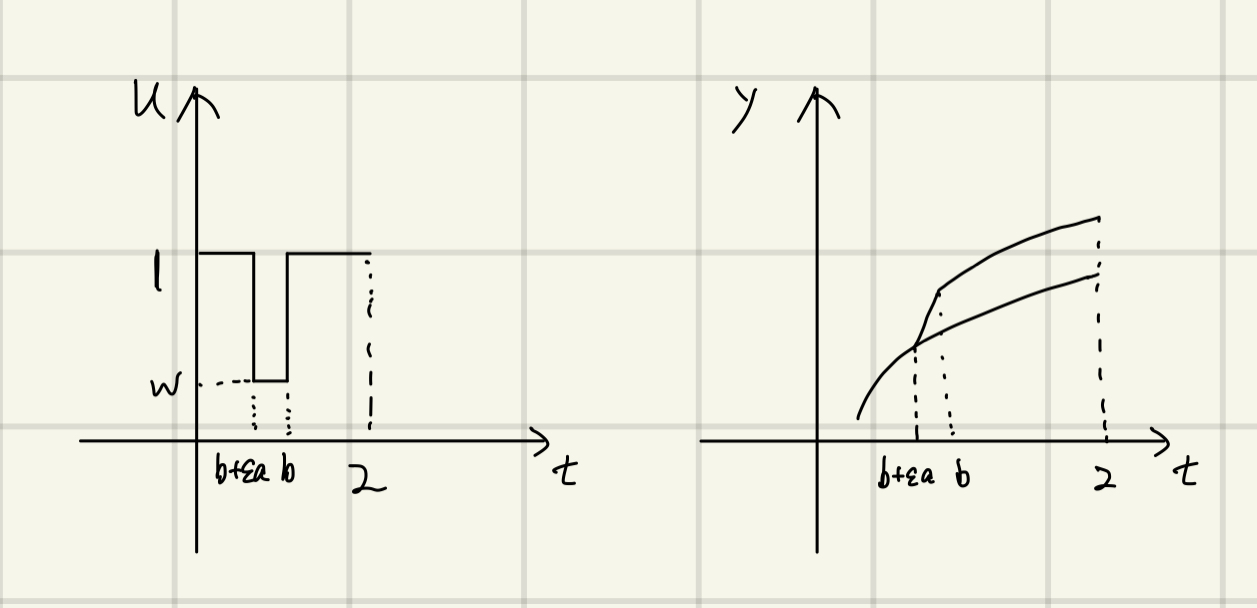
\includegraphics[width=\textwidth]{ECE553/hw6/IMG_0041.PNG}
    \caption{Spatial perturbation to the optimal control and its effect.}
    \label{fig:spatial_control_perturbation}
\end{figure}
\paragraph{Variational equation.} Numerical evaluation gives that $A_*(t) = \begin{bmatrix}0&0&0\\0&0&1\\0&0&0\end{bmatrix}$ and $\Phi(t^*,b) = e^{A_* (t^*-b)} = \begin{bmatrix}1&0&0\\0&1&2-b\\0&0&1\end{bmatrix}$. Possible spatial perturbation directions of $\delta(w,I) = \Phi(t^*,b)\nu_b(w)a$ are $\begin{bmatrix}0\\-t\\-1\end{bmatrix}$, $\forall t \in [0,2]$.
\paragraph{Terminal cone.} The terminal cone is shown in Fig.~\ref{fig:terminal_cone}.
\begin{figure}[H]
    \centering
    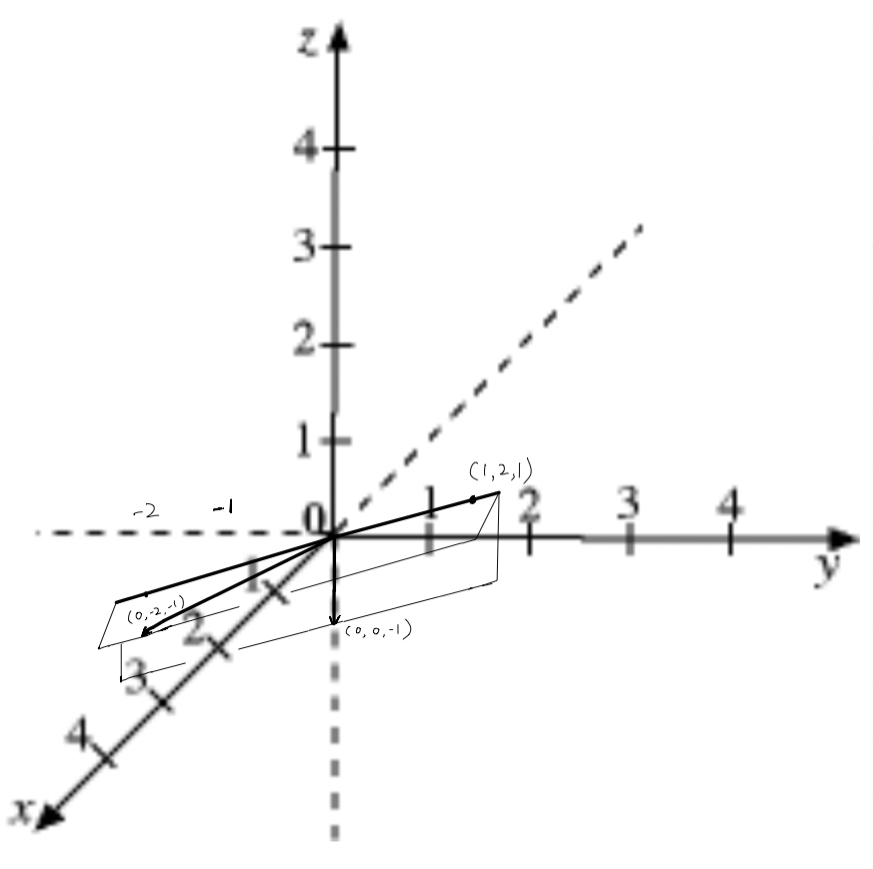
\includegraphics[width=\textwidth]{ECE553/hw6/IMG_0039.PNG}
    \caption{Terminal cone.}
    \label{fig:terminal_cone}
\end{figure}
\paragraph{Separating hyperplane.} As shown in Fig.~\ref{fig:terminal_cone}, we can chose $\begin{bmatrix}p_0^*\\p_1^*(t^*)\\p_2^*(t^*)\end{bmatrix} = \begin{bmatrix}0\\-1\\2\end{bmatrix}$.
\paragraph{Adjoint equation.} The adjoint equation is
\begin{align*}
& \dot{p}_0 = 0\\
& \dot{p} = \begin{bmatrix}0\\-p_1\end{bmatrix}.
\end{align*}
Using the boundary condition we have that $p_0 \equiv 0$, $p_1 \equiv -1$ and $p_2^*(t) = t$.
\paragraph{Properties of the Hamiltonian.} Since $p_2^* > 0$, $\forall t \in [0,2]$, $u^* \equiv 1$ satisfies the maximization condition. Second, $H|_* = -x_2(t) + t \equiv 0$.
\section*{Exercise 4.5}
Since there exists a continuous map from $B_\epsilon$ to $\tilde{B}_\epsilon$, we know that $\tilde{B}_\epsilon$ is homotopy-equivalent to $B_\epsilon$. Thus, there is no hole inside $\tilde{B}_\epsilon$. Furthermore, it is clear that the boundary of $\tilde{B}_\epsilon$ must be outside the ball at $\hat{y}_\epsilon$ with radius $\epsilon - o(\epsilon)$. Together with the fact that there is no hole inside $\tilde{B}_\epsilon$, we have that $\tilde{B}_\epsilon$ contains, for $\epsilon$ small enough, a ball centered at $\hat{y}_\epsilon$ whose radius is of order $\epsilon - o(\epsilon)$. Thus $\tilde{B}_\epsilon$ and $\overrightarrow{\mu}$ have non-empty intersection for small enough $\epsilon$.

\section*{Exercise 4.8}
We reduce this problem to Basic Variable-Endpoint Control Problem by adding an variable for time and writing down the new Lagrangian considering the terminal cost. The dynamics is
\begin{align*}
& \dot{x} = f(t, x, u),~~ x(0) = x_0,\\
& \dot{x}_{n+1} = 1,~~~~~~~ x_{n+1}(0) = t_0.
\end{align*}
The targe set is $[t_0, \infty) \times S_1 \times [t_0, \infty)$. The Lagrangian is $\bar{L} = L+\langle K_x, f \rangle$.

Then, for the maximum principle for the original problem, the Hamiltonian is $H(t,x,u,p,p_0) = \langle p, f \rangle + p_0 L$. First, we lose the condition that $H$ is $0$. We can only reach the differential equation 
\[
\frac{d}{dt} H|_* = H_t|_*.
\] Second, the transversality condition has to be updated. For the Basic Variable-Endpoint Control Problem, the transversality condition is
\[
\langle \bar{p}^*(t^*), d \rangle = 0, ~\forall d \in T_{x^*(t^*)}S_1.
\]
Following the derivation of Eq.~(4.45), we have that $p^*(t) := \bar{p}^*(t) - p_0^* K_x(x^*(t))$.
Thus, for the original problem, the transversality condition is that
\[
\langle p^*(t)+p_0^* K_x(x^*(t)), d \rangle = 0, ~\forall d \in T_{x^*(t^*)}S_1.
\]
\section*{Exercise 4.15}
Consider the following dynamics
\begin{align*}
&\dot{x}_1 = x_2,\\
&\dot{x}_2 = u,\\
&\dot{x}_3 = x_1^2.
\end{align*}
Then, the Hamiltonian is $H = p_1 x_2 + p_2 u + p_3 x_1^2 + p_0$. Applying the maximum principle, we have
\begin{align*}
&\dot{p}_1 = -2 p_3 x_1,\\
&\dot{p}_2 = -p_1,\\
&\dot{p}_3 = 0,
\end{align*}
which implies that $p_3$ is a constant and these differential equations resemble Eq.~(4.68). Again, we have that the switching function $\varphi(t) = p_2^*(t)$. Following the derivation in the textbook, we know that singular arcs are ruled out and $p_2^*(t)$ has infinitely many zeros. Projected onto the $x_1 - x_2$ plane, the new system is equivalent to the one in Sec.~4.4.4.

Furthermore, since the time intervals between consecutive switches decrease in geometric progression, the integral of $x_1^2$ is finite. We can just set $x_3(0)$ to the opposite of this integral. Then, the state will converge to $0$ in finite time but with infinitely many switchings.
\end{document}
